\documentclass{beamer}   % [notes=show,handout]

\usepackage{tikz}
\usepackage{graphicx}
\usepackage{hyperref}
\mode<presentation>

\usetheme{Frankfurt}%
\usecolortheme{seagull}

\definecolor{garnet}{RGB}{136,0,0}
\definecolor{clarksonGreen}{RGB}{0,52,21}

\setbeamercolor{palette primary}{fg=garnet,bg=white}
\setbeamercolor{palette secondary}{fg=clarksonGreen,bg=white}
\setbeamercolor{palette tertiary}{fg=clarksonGreen,bg=white}
\setbeamercolor{palette quaternary}{bg=clarksonGreen,fg=white}
\setbeamercolor{block title}{fg=black,bg=black!15}
\setbeamercolor{block body}{fg=black,bg=black!10}
\setbeamercolor{titlelike}{bg=garnet,fg=white} % parent=palette quaternar

\setbeamertemplate{footline}{\hspace*{.5cm}\scriptsize{\insertauthor
\hspace*{50pt} \hfill\insertframenumber\text{/}\inserttotalframenumber\hspace*{.5cm}}}

\newcommand{\R}{\mathbb{R}}


\begin{document}



\part{Introduction}
\lecture{Introduction}{Introduction}


\title{Modeling Human and Deer Interaction}
\subtitle{Actuarial Considerations}

\author{Liu, Sweeney, Zhou}
\institute{SUNY Potsdam and Clarkson University REU \\ with Dr. Kelly Black}
\date{July 30, 2013}

\begin{frame}[plain]
  \titlepage
  \begin{center}
  
\includegraphics[width=0.2\textwidth]{SUNYPotsdam}
  
\includegraphics[width=0.1\textwidth]{nsf_logobig}
  
\includegraphics[width=0.15\textwidth]{clarksonGreen}
\end{center}
\end{frame}

\begin{frame}
  \frametitle{Outline}
  \vspace{-5mm}
  \tableofcontents[]
\end{frame}



\section{Introduction}

\begin{frame}
 	\begin{center}
 	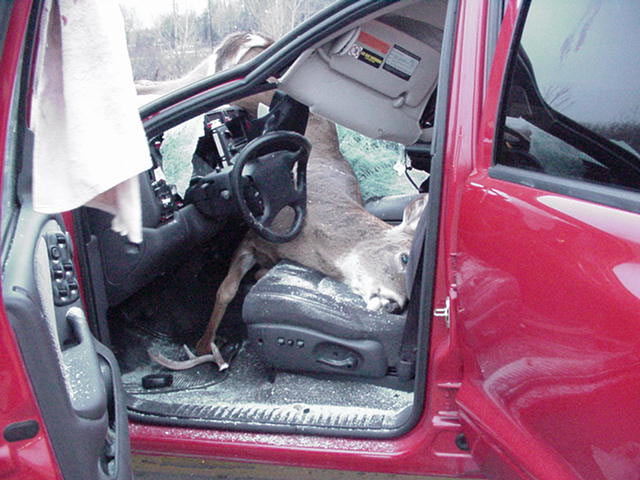
\includegraphics[height=7cm]{DeervsDurango}
 	\end{center}
\end{frame}

\begin{frame}
    \frametitle{Background}
In the U.S., between July 1, 2011 and June 30, 2012:
    \begin{itemize}
    	\item 1.23 million deer-vehicle collisions occurred.
    	\item Costs are more than \$4 billion in vehicle damage.
    	\item The average claim for deer-vehicle collisions was \$3,305 per accident.
    	\item The Insurance Institute for Highway Safety (IIHS) noted that deer-vehicle collisions in the U.S. cause about 200 fatalities annually.
    \end{itemize}
\emph{(State Farm, Insurance Journal)}
\end{frame}


\begin{frame}
    \frametitle{Question?}
How do insurance companies manage funds associated with deer vehicle collisions?
\end{frame}


\section{Population Biology}

\begin{frame}
    \frametitle{Deer Population}
    \begin{itemize}
    	\item Assumptions
		\begin{itemize}
    		\item Population is near carrying capacity.
    		\item The only predation is human i.e. hunting and car fatalities.
    		\item Migrations rates are balanced across counties.
		\item Customers of one insurance company experience the same collision rate as the general population.
    		\end{itemize}
    \end{itemize}
\end{frame}

\begin{frame}
    \frametitle{Logistic Equation with Harvest}
	\vspace{-1cm}
	\begin{eqnarray*}
		\frac{dx}{dt} &=& rx \left( 1-\frac{x}{f} \right) -hx
	\end{eqnarray*}
	\begin{itemize}
		\item $f$ - Carrying capacity
		\item $r$ - Growth rate
		\item $h$ - Harvest rate
	\end{itemize}
\end{frame}

\begin{frame}
    \frametitle{Rescaling the Logistic Equation with Harvest}
	\vspace{-1cm}
	\begin{eqnarray*}
		\frac{dx}{dt} &=& rx \left( 1-\frac{x}{f} \right) -hx\\
		 &=& rx-\frac{rx^{2}}{f}-hx\\
		 &=& (r-h)x-\frac{rx^{2}}{f}\\
		 &=& (r-h)x \left(1-\frac{rx^{2}}{f(r-h)} \right)\\
		 &=& \tilde{r}x \left( 1-\frac{x}{\tilde{f}} \right)		
	\end{eqnarray*}
\end{frame}

\begin{frame}
    \frametitle{Athens County, Ohio}
Schwabe, \emph{et al.}, 2000
	\begin{itemize}
		\item Carrying capacity is approximately 28,000
		\item Growth rate is 1.7
		\item Harvest rate is 0.16
	\end{itemize}
\end{frame}






\section{Insurance}

\begin{frame}
    \frametitle{State Regulations and Bond Funds}
%%%%%%%%%%%%% How insurance companies work
	\begin{itemize}
		\item Low risk government bonds
		\item Premiums from customers
		%%%%% AREA WHERE YOU LIVE AKA DEER, driving record, age, type of car
		\item Claims based on accidents
	\end{itemize}
\end{frame}



\section{Modeling}

We discuss the model employed to describe the population of deer and
the associated bond fund used to balance the liabilities associated
with claims that result from deer and automobile collisions. -- give
an overview and outline for this section --

Overview of the issues and motivation.




%%% Local Variables: 
%%% mode: latex
%%% TeX-master: "deerFundModeling"
%%% End: 




\section{Results}

Discuss the results here. They are FABULOUS!

%%% Local Variables: 
%%% mode: latex
%%% TeX-master: "deerFundModeling"
%%% End: 





\section{References}

\begin{frame}
    \frametitle{References}

\begin{thebibliography}{3}

\bibitem{higham}
Higham, D. J., 2001:
An Algorithmic Introduction to Numerical Simulation of Stochastic Differential Equations.
\emph{SIAM review},
\textbf{43(3)}, 525-546.

\bibitem{schwabe}
Schwabe, K. A., Schuhmann, P. W., Tonkovich, M. J., \& Wu, E., 2000:
An Analysis of Deer-Vehicle Collisions: the Case of Ohio.
\emph{Human Conflicts with Wildlife: Economic Considerations}.

\bibitem{skiadas}
Skiadas, C. H., 2001:
Exact Solutions of Stochastic Differential Equations: Gompertz and Generalized Logistic.
\emph{Methodology and Computing in Applied Probability},
\textbf{12}, 261-270.

\end{thebibliography}

\end{frame}



\section{Acknowledgments}

\begin{frame}
    \frametitle{Acknowledgments}
	Thanks to Dr. Joel Foisy, Dr. Kelly Black and NSF (NSF \# 1262737) for their support and involvement in this program.
\end{frame}



\end{document}
